\documentclass[12pt, twoside]{report}
\usepackage[utf8]{inputenc}
\usepackage[a4paper,width=150mm,top=25mm,bottom=25mm,bindingoffset=6mm]{geometry}
\usepackage{graphicx}
\usepackage{listings}
\usepackage[backend=bibtex, style=authoryear, maxcitenames=2]{biblatex}
\addbibresource{references.bib}
\usepackage{cleveref} % cleverref has to be loaded after hyperref!


\begin{document}

\begin{titlepage}
    \begin{center}
        \vspace*{1cm}
        
        \Huge{\textbf{Extracting recipe ingredients from cookbooks}}
        
        \vspace{1cm}
        
        \Large{by}\\
        \LARGE{Torsten Knauf}
        
        \vspace{1cm}
        
        \Large
        A thesis presented for the degree of\\
        Master of Science
        
        \vspace{1cm}
        
        
\includegraphics[width=0.4\textwidth]{Images/cau-siegel.pdf}
        
        Research Group for Communication Systems\\
        \large{at} \\
        Faculty of Engineering\\
        Christian-Albrechts-Universität zu Kiel\\
        Germany\\
        31.03.2017
    \end{center}
    
    \vspace{1cm}
    
    \LARGE
    \begin{tabbing}
    Supervisor: \= Prof. Dr.-Ing.Norbert Luttenberger\\
    \> Dr.-Ing. Jesper Zedlitz
    \end{tabbing}
\end{titlepage}

\pagenumbering{Roman}
\chapter*{Abstract}
Always do this one last, when knowing the things to praise  yourself for :P

\chapter*{Acknowledgements}
If I don't profit from nice people in these thesis, I have done something horrible wrong. So try to remember most of them here at the end... :)

\tableofcontents

\listoffigures
\listoftables
\lstlistoflistings

\clearpage
\pagenumbering{arabic}  
\chapter{Introduction}
A recipe parser, which can tag old and rather unstructured cookbooks according to the ontology of \parencite{schemaRecipe}, is developed in this thesis. Once it is tagged, it is easy to extract the tagged entities. The parser is developed and tested with \textit{Davidis, Henriette: Praktisches Kochbuch für die gewöhnliche und feinere Küche. 4. Aufl. Bielefeld, 1849} but can be adapted easily to every German cookbook. For other languages new training data and dictionaries for the machine learning preparation of the parser have to be provided, but the general algorithm can be inherited.

This effort is motivated by nutritional science. Being able to extract the ingredients of a recipe automatically simplifies research according healthy food as well as historical analysis.

The thesis is structured as follows:


\chapter{Making a cookbook machine-readable}
This chapter covers shortly how we transform a cookbook in a machine-readable XML file, which can be processed further arbitrarily. To achieve this, the cookbook has to be digitalized first and afterwards enriched through an ontology.

\section{Digitalisation}
In general there are two different ways, how to digitalize a book. The first one is to scan each side and let an \textit{optical character recognition}-program translate the scanned pictures into text. The second one is to \textit{type it manual} into a computer.

The German Text Archive provides a collection of German texts from 16th to 19th century including \textit{Davidis, Henriette: Praktisches Kochbuch für die gewöhnliche und feinere Küche. 4. Aufl. Bielefeld, 1849} in \parencite{DTA}. They digitalized it through double keying, meaning that two people manual typed the book into the computer. Differences in their versions were revised by a third person.

The digitalized version can be downloaded from \parencite{DTA}. It is already enriched through \textit{TEI: Text Encoding Initiative}-standard\footnote{http://www.tei-c.org/index.xml}. TEI is a standard for representing text in digital form, which should be analysed later in humanities, social sciences or linguistics.

Figure XXX depicts the digitalized version of our cookbook.

Because we are only interested in extracting certain data from the recipes and not in linguistic analysis or something else, we transformed the digitalized version as depicted in figure XXX. The essence of this version is, that every recipe can be easily transformed into this form and that every recipe can be easily read by human for manual tagging. 

\section{CueML ontology}
For general automatic extraction and further processing of information an ontology is needed. In computer science an ontology is a vocabulary with defined meaning. A very nice description for the use of ontologies, which are a requirement for the Semantic Web, can be found in \parencite{semanticWeb}.

\parencite{schemaRecipe} is an existing ontology for recipes. Figure XXX depicts its usage. It works fine for well structured recipes, which already have a list of used ingredients. However it is not well suited for tagging our cookbook as the following example demonstrates.

Therefore we invented \textit{cueML}...

Now this format can be easily transformed into a well structured recipe and afterwards be tagged with the standard ontology from \parencite{schemaRecipe}


\section{Need for automatisation}
\parencite{manualTagging} error prone. Brauche so lange pro Rezept


\chapter{Related Work}
In general there exists many effort about extracting useful information from textual and unstructured resources. The superordinate term for this field of research is \textit{Text Mining}. It was first mentioned in \parencite{KDT} and on overview can be found in \parencite{surveyOfTextMining}. 

The algorithms for extracting useful information depend highly on existing semi-structures, which can be taken advantage of. Here we present existing algorithm, which we found in the domain of cooking, and distinct their effort from this thesis.

\section{Skip The Pizza}
\parencite{REgutGenug} is a project described on WordPress.org. The author wants to combine his two hobbies cooking and software engineering. For being able to answer questions like "How many ingredients does a typical recipe consist of?" or "Which are the most frequent ingredients?", he extracts the ingredients of recipes from http://recipes.wikia.com/wiki/Recipes\_Wiki.

\begin{lstlisting}[frame=single, basicstyle=\footnotesize\ttfamily,caption={Shortened example recipe from \\ http://recipes.wikia.com/wiki/Recipes\_Wiki}, label=lst:recipeWiki]
    * Makes 6 to 8 servings

== Ingredients ==
* 2 tbsp extra virgin [[olive oil]]
* 3 cloves [[garlic]], finely chopped
[...]

== Directions ==
Heat olive oil and garlic in large skillet over low heat until
garlic begins to sizzle.
Add tomatoes, [...]

[[Category:Cathy's Recipes]]
[[Category:Garlic Recipes]]
[...]
\end{lstlisting}

The recipes have the internal structure of \cref{lst:recipeWiki}. The semi-structure, that after \texttt{== Ingredients ==} comes a list of ingredients, can be recognized easily. Per line is one ingredient enclosed within \texttt{[[ingredient name]]}. Using this semi-structure a regular expression is already good enough for extracting the ingredients from these recipes.

 
\section{Domain Specific Information Extraction for Semantic Annotation}
\parencite{GrammaBased} is a diploma thesis about extracting ingredients and their further processing from recipes. Their algorithm could be divided into two main parts.

One main part is to check every word if it is occurs in a dictionary of ingredients respectively a dictionary of actions and tag it accordingly. For keeping the dictionaries as small as possible they do a morphological Analysis and only store the lemmas of the words. The second main part, and more sophisticated task, is to identify which action should be applied to which ingredient. They have two different approaches for that.

\textbf{The first one} is to do a part of speech tagging and afterwards trying to apply a small set of rules. The example rule 1 means apply the action to all following ingredients and gets matched. Therefore it is extracted that buttermilk and bananas should be extracted.

\begin{lstlisting}[frame=single, basicstyle=\footnotesize\ttfamily,caption={Rule based example}, label=lst:ruleBased]
add buttermilk and bananas
->
add[ACT] buttermilk[ING] and[CC] bananas[ING]
->
rule 1: VP -> ACT NP (,NP)* (CC NP)?
   -> ACT NP CC NP			und Hilfsregel:  NP -> DT? JJ* ING
   -> ACT ING CC ING

\end{lstlisting}

\textbf{The second one} is to do a dependency based parsing, which represent the semantic structure of a sentence in a tree like format.

\begin{figure}[h]
	\centering
	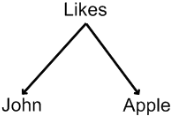
\includegraphics[]{Images/JohnLikesApple}
	\caption{John likes apple \parencite{GrammaBased}}
	\label{fig:johnLikesApple}
\end{figure}

For example \cref{fig:johnLikesApple} represents, that the subject of like is John and the liked object is apple.
The format as well as building the tree is way more complex than the previous simple rules, but the tree can be build by already existing tools like the Standfod Parser\footnote{http://nlp.stanford.edu/software/lex-parser.shtml}. Having the semantic structure of the sentences, it is trivial to extract which action should be applied to which ingredient.


\section{Extracting Structured Data From Recipes Using Conditional Random Fields}

\section{Distinction to this work}



\chapter{Development of recipe parser}

\section{Overall picture}
\subsection{workflow}
\subsection{preparation}
\subsection{evaluation}
-Precision -Recall F-measure

\section{First Iteration: Basis CRF}
Git-tag
\subsection{Idea}
\subsection{Evaluation}

\section{Final recipe parser}
\subsection{Workflow}
\subsection{Evaluation}

\chapter{Discussion}
- Übertragung auf beliebige Bücher (Wenn Buch hat bereits Zutatenliste erste Phase entfällt)
- TDD / früh Plausibilitäts-Überprüfungen (insbesondere fürs Schemata, Mengenangaben historische Recherche nötig)

\section{Power of machine readable data}
Machine readable data are very powerful. But \textit{with great power comes great responsibility}\footnote{A well known proverb which probably has its origin from the French National Convention during the period of French Revolution. \parencite{quoteInvestigator}}. In the context of a recipe parser this might be a little bit exaggerated. But specially in mind of the global surveillance disclosures denounced by Edward Snowed with still uncertain dimension, I think it is important to have a consciousness for what can be done. Therefore I want to think about, what can be done through innocent looking machine readable tags. 
\bigskip

\textbf{For the good} there exists already much effort for services, which require being able to extract ingredient from recipes.

 (e.g. \cite{ingredientNetworks} or \cite{recipeRecommendation}).

Further more, having a huge machine-readable base of recipes and its ingredients, can also provide insights in sociological research. For example in (((Flavor network and the principles of food pairing : Scientific Reports))) is a comparison between American and Asian kitchen based on about 56.000 recipes.

There are many more interesting questions, which could be analysed like a historic analysis of the development and changes of cooking. Occurrences of non-local ingredients or meals are evidence for inter cultural exchange and globalisation. More expensive ingredients could be an indication for prosperity, while very simple kitchen for poverty or even wartimes...
\bigskip

\textbf{In the bad} \parencite{clintonHealth} "schwacher vegetarier"


\chapter{Summary}


\appendix
\chapter{Statutory Declaration}
I declare that I have developed and written the enclosed Master Thesis completely by myself, and have not used sources or means without declaration in the text. Any thoughts from others or literal quotations are clearly marked. The Master Thesis was not used in the same or in a similar version to achieve an academic grading or is being published elsewhere.
\newline
\newline
\newline
\rule{\textwidth}{1pt}
Location, Date \hfill Signature 

\chapter{Something else}
hi

\chapter{Something else else}
hello

\printbibliography

\end{document}